\section{Preliminaries}\label{sads}
In this section, we give the definition of a streaming authenticated data structure (SADS), as introduced in the PSTY paper~\cite{DBLP:conf/eurocrypt/PapamanthouSTY13}.
We denote with $\lambda$ the security parameter and with $n=\mathsf{poly}(\lambda)$ an upper bound on the size of the stream. PPT stands for \emph{probabilistic polynomial-time} and $\negl(\lambda)$ is a negligible function, i.e., a function less than $1/\mathsf{poly}(\lambda)$, for all polynomials $\mathsf{poly}(\lambda)$. We define $[n]=\{0,1,\ldots,n\}$. 
\begin{defn}[SADS scheme]\label{define_sauth}
  Let $D$ be \emph{any} data structure that supports queries $q$ and
  updates $\mathsf{upd}$. An SADS scheme ${\bf A}$ is a collection of the following six PPT algorithms:
\begin{enumerate}
\item $\mathsf{pk}\leftarrow\mathsf{genkey}(1^\lambda,n)$: On
  input the security parameter $\lambda$ and an upper bound $n$ on the size of the stream, it outputs a public key $\mathsf{pk}$;

\item
  $\{\mathsf{auth}(D_0),d_0\}\leftarrow\mathsf{initialize}(D_0,\mathsf{pk})$:
  On input an empty data structure $D_0$ and the public key $\mathsf{pk}$, it computes the authenticated data structure $\mathsf{auth}(D_0)$ and the respective state $d_0$ of it;

\item
  $d_{h+1}\leftarrow\mathsf{updateVerifier}(\mathsf{upd},d_h,\mathsf{pk})$:
  On input an update $\mathsf{upd}$ to data structure $D_h$, the current state $d_h$ and the public key $\mathsf{pk}$, it outputs the updated state $d_{h+1}$;

\item
  $\{D_{h+1},\mathsf{auth}(D_{h+1})\}\leftarrow\mathsf{updateProver}(\mathsf{upd},D_h,\\ \mathsf{auth}(D_h),\mathsf{pk})$:
  On input an update $\mathsf{upd}$ to data structure $D_h$, the authenticated data
  structure $\mathsf{auth}(D_h)$ and the public key $\mathsf{pk}$, it
  outputs the updated data structure $D_{h+1}$ along with the updated
  authenticated data structure $\mathsf{auth}(D_{h+1})$;

\item
  $\{\alpha(q),\Pi(q)\}\leftarrow\mathsf{query}(q,D_h,\mathsf{auth}(D_h),\mathsf{pk})$:
  On input a query $q$ on data structure $D_h$, the authenticated data
  structure $\mathsf{auth}(D_h)$ and the public key $\mathsf{pk}$, it returns the
  answer $\alpha(q)$ to the query, along with a proof $\Pi(q)$;

\item $\{{\tt{1}},{\tt{0}}\}\leftarrow
   \mathsf{verify}(q,\alpha(q),\Pi(q),d_h,\mathsf{pk})$: On input a query $q$,
  an answer $\alpha(q)$, a proof $\Pi(q)$ for query $q$, a digest $d_h$ and the public key $\mathsf{pk}$,
  it outputs either $\tt{1}$ (accepts) or $\tt{0}$ (rejects);
  \end{enumerate}
\end{defn}
There is \emph{no secret key in our definition}, supporting in this way \emph{public verifiability}. There are two properties that an SADS scheme should satisfy, namely
\emph{correctness} and \emph{security} (as in signature
schemes definitions).

\begin{defn}[Correctness]\label{sound_def}
  Let ${\bf A}$ be an SADS scheme consisting of the set of algorithms. We say that the SADS
  scheme ${\bf A}$ is \emph{correct} if, for all $\lambda \in
  \mathbb{N}$, for all $\mathsf{pk}$ output by algorithm
  $\mathsf{genkey}$, for all $D_h,\mathsf{auth}(D_h),d_h$ output by one
  invocation of $\mathsf{initialize}$ followed by polynomially-many
  invocations of $\mathsf{updateVerifier}$ and \\
   $\mathsf{updateProver}$, where $h\ge 0$, for all queries $q$
  and for all $\Pi(q),\alpha(q)$ output by
  $\mathsf{query}(q,D_h,\mathsf{auth}(D_h),\mathsf{pk})$, with all but
  negligible probability $\negl(\lambda)$, it holds that ${\tt{1}}\leftarrow\mathsf{verify}(q,\Pi(q),\alpha(q),d_h,\mathsf{pk})$.
\end{defn}

Apart from the 6 algorithms in Definition~\ref{define_sauth}, we also define the algorithm $\{{\tt{0},\tt{1}}\}\leftarrow\mathsf{check}(q,\alpha,D_{h})$ such that it outputs ${\tt{1}}$ if and only if $\alpha$ is the correct answer to query $q$ on data structure $D_h$ (otherwise it outputs ${\tt{0}}$).  

\begin{defn}[Security]\label{sec_def_general}
  Let ${\bf A}$ be an SADS scheme, $\lambda$ be the security
  parameter, $D_0$ be the empty data structure and
  $\mathsf{pk} \leftarrow \mathsf{genkey}(1^{\lambda})$. Let also
  $\mathsf{Adv}$ be a PPT adversary and let $d_0$ be the state output by $\mathsf{initialize}(D_0,\mathsf{pk})$. 
\begin{itemize}
\item (Update) For $i=0,\ldots,h-1=\mathsf{poly}(k)$, $\mathsf{Adv}$ picks the update $\mathsf{upd}_i$ to data structure $D_i$. Let $d_{i+1}\leftarrow\mathsf{updateVerifier}$\\
$(\mathsf{upd}_i,d_i,\mathsf{pk})$ be the new state corresponding to the updated data structure $D_{i+1}$.
\item (Forge)  $\mathsf{Adv}$ outputs a query $q$, an answer $\alpha$ and a proof $\Pi$.
\item (Check)  $\mathsf{Adv}$ outputs a query $q$, an answer $\alpha$ and a proof $\Pi$.
\end{itemize}
 We say that the SADS scheme ${\bf A}$ is \emph{secure} if for all $\lambda \in \mathbb{N}$, for all
  $\mathsf{pk}$ output by algorithm $\mathsf{genkey}$,
  and for any PPT adversary $\mathsf{Adv}$ the following probability is negligible $\negl(\lambda)$.
\[
\label{lab:prob_sec}
\Pr\left[
\begin{tabular}{rl}
    $\{q,\Pi,\alpha\}\leftarrow\mathsf{Adv}(1^{\lambda},\mathsf{pk});$&${\tt{1}}\leftarrow \mathsf{verify}(q,\alpha,\Pi,d_h,\mathsf{pk});$\\
    &${\tt{0}}\leftarrow\mathsf{check}(q,\alpha,D_{h}).$
  \end{tabular}\right]\,.
\]
\end{defn}
\subsection{Generalized Hash Trees}
Recall that a Merkle hash tree~\cite{m-cds-89} is a labeled binary tree $T$ where the label $\lambda(w)$ of every node $w$ is the collision resistant hash (e.g., a SHA-2 hash) of the labels $\lambda(u)$ and $\lambda(v)$ and of its children $u$ and $v$, i.e., $\lambda(w)=h(\lambda(u),\lambda(v))$. When function $h$ is applied recursively on all the nodes of the tree, the label $\lambda(r)$ of the root $r$ has the following property: A PPT adversary cannot find two different data sets at the leaves that produce the same label at the root of a Merkle tree.

However, certain hash functions have different domain and range. E.g., in SWIFFT~\cite{swifft}, the input is a binary vector while the output value is in a finite filed. Obviously, we cannot employ such hash functions in a traditional Merkle hash tree. Generalized hash trees, introduced in the PSTY paper, provide a way to overcome this domain-range discrepancy problem.







Let $h: \mathcal{D}\times \mathcal{D}\rightarrow \mathcal{R}$ be a collision resistant hash function accepting two inputs that take values from domain $\mathcal{D}$ and outputting a value in a \emph{different} range $\mathcal{R}$. Let $u$ and $v$ be the two children of $w$ with labels $\lambda(u)$, $\lambda(v)$ and $\lambda(w) \in \mathcal{D}$. Instead of applying hash functions on node labels directly, generalized hash trees use a \emph{deterministic} and \emph{easily computable} projection function $\phi: \mathcal{D}\rightarrow \mathcal{R}$, such that $\phi(\lambda(w))=h(\lambda(u),\lambda(v))$.

%Generalized hash trees require that the labels $\lambda(u)\in \mathcal{D}$ and $\lambda(v)\in \mathcal{D}$ of the children $u$ and $v$ hash to a \emph{deterministic} and \emph{easily computable} projection function $f: \mathcal{D}\rightarrow \mathcal{R}$ of the label $\lambda(w)\in \mathcal{D}$ of the parent $w$, i.e., $f(\lambda(w))=h(\lambda(u),\lambda(v))$.
%\begin{equation}\label{main_generalized}
%\end{equation}

Clearly, the labeling of a generalized hash tree need \emph{not} to be unique: In the above example, $\lambda(w)$ can be any $\phi$-preimage of $h(\lambda(u),\lambda(v))$. However, the collision resistant property of Merkle trees is still true: Any two valid hash trees representing different data sets at the leaves but with the same root label yield a collision to the underlying hash function. We now formally define generalized hash trees.
\begin{defn}[Full binary tree]\label{full_bin_def}
A \emph{full binary tree} $T$ is a non-empty tree where every internal node has two children. It is represented with set of binary strings, where $\epsilon$ is the empty string representing the root of $T$ and $w0$ and $w1$ are the string representations of the left and right children of a node having string representation $w$. 
\end{defn}

For example, a full binary tree with five nodes is $T=\{\epsilon,0,1,00,\\01\}$. Note that full binary trees need not be complete, i.e., not all leaves must lie at the same level.
\begin{defn}[Labeled binary tree]
A \emph{labeled binary tree} $(T,\lambda)$ is a full binary tree $T$ along with labels $\lambda(w)$ for all $w\in T$. 
\end{defn}

\begin{defn}[Generalized hash tree]\label{def_generalized}
Let $h: \mathcal{D}\times \mathcal{D}\rightarrow \mathcal{R}$ be the hash function, and $\phi: \mathcal{D}\rightarrow \mathcal{R}$ be the projection function. A \emph{generalized hash tree} $(T,\lambda,\phi,h)$ is a labeled binary tree $(T,\lambda)$ such that \textbf{(a)} for all $w\in T$, $\lambda(w)\in \mathcal{D}$; \textbf{(b)} for all internal nodes $w\in T$, $\phi(\lambda(w))=h(\lambda(w0),\lambda(w1))$,
where $w0$ and $w1$ are the left and right children of $w$ respectively.% Moreover we say that $(T,\lambda,\phi,h)$ is \emph{collision resistant} with respect to $h$ if $h$ is collision resistant.
\end{defn}
%\begin{definition}[Distinct generalized hash trees]\label{distinct-trees}
%Two generalized hash trees $(T,\lambda,\phi,h)$ and $(T,l,f,h)$ are \emph{distinct} if and only if $\lambda(\epsilon)=l(\epsilon)$ (where $\epsilon$ is the root of $T$) and there exists $w\in T$ such that $\lambda(w)\ne l(w)$.
%\end{definition}

\begin{defn}[Tree collision]\label{distinct-trees}
A \emph{tree collision} is a pair of two distinct generalized hash trees $(T,\lambda,\phi,h)$ and $(T,l,\phi,h)$ such that $\lambda(\epsilon)=l(\epsilon)$.
\end{defn}

The next main security theorem establishes the collision resistance for generalized hash trees. Please refer to the PSTY work~\cite{DBLP:conf/eurocrypt/PapamanthouSTY13} for a detailed proof.
\begin{theorem}[Collision resistance]\label{col_res}
Let $\lambda$ be the security parameter, $T$ be a full binary tree of $\mathsf{poly}(\lambda)$ depth. If $h$ is collision resistant, there is no PPT algorithm that can output a tree collision $(T,\lambda,\phi,h)$ and $(T,l,\phi,h)$, except with probability $\negl(\lambda)$.
\end{theorem}

\subsection{The generalized hash trees for SADS}
For the SADS, we need an extension of the full binary tree from Definition~\ref{full_bin_def} that can store values at its leaves. 
\begin{defn}[Structured binary tree]\label{structured_binary}
Let $M$ be a \\
power of two. A \emph{structured binary tree} $T_\mathcal{C}$ is a full binary tree $T$ of $\log M$ levels where all the leaves lie at the last level of the tree, storing values $\mathcal{C}=[c_0,c_1,\ldots,c_{M-1}]$, where $c_i\in [n]$.  
\end{defn}
In a structured binary tree, each leaf corresponds to an element in the universe of the stream. The sequence of elements (from leftmost to rightmost) form an ordered universe. E.g., let the universe of a structured binary tree with $8$ leaves be $\{0,1,\ldots,7\}$. The leaves from left-to-right correspond to elements $0,1,\ldots,7$. Without loss of generality, we will assume the universe of size $M$ is $\{0,1,\ldots,M-1\}$. The value stored at each leaf indicates the frequency of the corresponding leaf element. E.g., in a structured binary tree of $8$ leaves, $c_6$ indicates the frequency of element $6$.

\subsection{Groups and homomorphisms}
We now give a brief review on groups and homomorphism that are going to be needed for defining our abstract construction. Please refer to~\cite{algebrabook} for a comprehensive study. 

A {\it commutative group} is a set $\mathcal{G}$ with an operation $\odot$, such that (1) the operation $\odot$ is associative and commutative; (2) $\mathcal{G}$ has an identity; (3) Every element in $\mathcal{G}$ has an inverse. We use $0_{\mathcal{G}}$ to denote the identity and use $\sum \in \mathcal{G}$ to denote the summation over group $\mathcal{G}$. A subset ${\mathcal{H}}$ of ${\mathcal{G}}$ is a {\it subgroup} of ${\mathcal{G}}$ if ${\mathcal{H}}$ forms a group under the same operation $\odot$. A subgroup ${\mathcal{N}}$ of group ${\mathcal{G}}$ is a {\it normal subgroup} if it is invariant under conjugation; that is, $\forall n \in {\mathcal{N}}$, $\forall g \in {\mathcal{G}}$,  $g \odot n \odot g^{-1} \in  {\mathcal{N}}$.

In this paper, we focus on the two commutative groups with respect to the {\it domain} and the {\it range}. Namely, let $\mathcal{D}$ be the domain with an operation $\oplus$, and $\mathcal{R}$ be the range with an operation $\otimes$.

A {\it homomorphism} $\phi: \mathcal{D} \rightarrow \mathcal{R}$ is a map from $\mathcal{D}$ to $\mathcal{R}$ such that for all $x, y$ in $\mathcal{D}$, $\phi(x \oplus y) = \phi(x) \otimes \phi(y)$. The {\it kernel} of the homomorphism $\phi$ is the set of elements in $\mathcal{D}$ that are mapped to the identity in $\mathcal{R}$:  $ker ( \phi)=\{x \in \mathcal{D}\, | \, \phi(x)=0_{\mathcal{R}}  \}$. Notice $ker(\phi)$ is a normal subgroup of $\mathcal{D}$ and always contains $0_{\mathcal{D}}$, i.e., $\phi(0_{\mathcal{D}}) = 0_{\mathcal{R}}$. The {\it image} of the homomorphism $\phi$ is $im (\phi) = \{\phi(x)\,| \, x \in \mathcal{D}\}$. The homomorphism $\phi$ is surjective if and only if $im ( \phi) = \mathcal{R}$.

An {\it isomorphism} is a bijective group homomorphism. Two groups $\mathcal{D}$ and $\mathcal{R}$ are {\it isomorphic} if there exists an isomorphism from one to the other.

Let $H$ be a subgroup of $\mathcal{D}$ and $a \in \mathcal{D}$. The subset $coset(a,H) =\{a \oplus h \,| \, h \in H\}$ is called a {\it coset} of $H$. For a normal subgroup $N \in \mathcal{D}$, the {\it quotient group} $ \mathcal{D} / N$ is defined as the set of cosets of $N$ in $\mathcal{D}$: $\mathcal{D} / N=\{coset(a,N) | a\in \mathcal{D}\}$. 

Let $\phi: \mathcal{D} \rightarrow \mathcal{R}$ be a surjective group homomorphism. The first isomorphism theorem states that 
the quotient group $\mathcal{D} / ker(\phi)$ is isomorphic to $\mathcal{R}$~\cite{algebrabook}.

For example, let $\phi: \mathbb{C} \rightarrow \mathbb{R}$ be the mapping from every complex number to its absolute value. It is easy to check $\phi$ forms a homomorphism under multiplication. The kernel of $\phi$ is the unit circle $U$, as it maps to the multiplication identity $1$ in $\mathbb{R}$. The quotient group $\mathbb{C} / ker(\phi)$ consists of all multiples of $U$. In other words, it is the collection of all circles centered at the origin in $\mathbb{C}$, each of which is a coset of $U$. Clearly, there is a bijection between each circle in $\mathbb{C}$ and its radius in $\mathbb{R}$. 

%\babis{please develop the last two paragraphs a bit more. Could you please give an example where you specify a two groups, a $\phi$ and then you show that $\phi$ from $\mathcal{D} / ker(\phi)$ is isomorphic to $\mathcal{R}$.}

%In the following sections, we instantiate the generalized hash tree for a structured binary tree using the lattice-based hash function %$h_{n}(\vc{x},\vc{y}) = \vc{L}\cdot\vc{x}+\vc{R}\cdot \vc{y}$ from Definition~\ref{hash_function_b}, where $\mathcal{D}=[n]^m$ and \mathcal{R}=\mathbb{Z}_q^k$---see Section~\ref{lattices-section} for the definition of all parameters $k,n,m,q$. We will also show which projection function $f$ to use and how to compute the labels $\lambda$ so that Definition~\ref{def_generalized} is satisfied.

\section{Abstract construction}\label{abstract_construction}
In this section, we define the hash function, the projection function and the labeling function for our abstract SADS construction. See Definitions~\ref{hashfunction},~\ref{projection} and~\ref{main_expression} respectively. 

\noindent {\bf The class of hash functions.}
We characterize the class of hash functions that fit our abstract SADS. Let $\mathcal{D}$ and $\mathcal{R}$ be the domain and the range of interest, both of which are commutative groups.
\begin{defn}[hash function]\label{hashfunction}
The class of hash functions of SADS, $h: \mathcal{D} \times \mathcal{D} \to \mathcal{R}$ is characterized as follows:
\begin{enumerate}
\item $h({\bf x, y}) = {\bf {\cal H}_{L}(x)} \otimes {\bf {\cal H}_{R}(y)}$.
\item There is no PPT algorithm can find $\bf x_{\delta}, y_{\delta} \neq 0_{\mathcal{D}}$ such that $\bf {\cal H}_{L}(x_{\delta}) + {\cal H}_{R}(y_{\delta})= {\bf 0}_{\mathcal{R}}$ with non-negligible probability.\label{CR}
\item For ${\bf x,y} \in \mathcal{D}$, ${\bf {\cal H}_{A}}({\bf x \oplus y}) ={\bf {\cal H}_{A}}({\bf x}) \otimes {\bf {\cal H}_{A}}({\bf y})$,  where $\bf A$ is either $\bf L$ or $\bf R$.
\end{enumerate}
\end{defn}

\begin{corol}
The hash function $h$ in Definition~\ref{hashfunction} is collision resistant.
\end{corol}
\begin{proof}
Assume there is a PPT algorithm $A$ that outputs two distinct pairs of $ ({\bf x}_{1},{\bf y}_{1}), \, ({\bf x}_{2}, {\bf y}_{2}) $ $\in \mathcal{D}$, such that $${\bf {\cal H}_{L}}({\bf x}_{1}) \otimes {\bf {\cal H}_{R}}({\bf y}_{1}) ={\bf {\cal H}_{L}}({\bf x}_{2}) \otimes {\bf {\cal H}_{R}}({\bf y}_{2})$$with non-negligible probability. Then, the PPT algorithm can find $\bf x_{\delta}, y_{\delta} \neq 0_{\mathcal{D}}$ s.t. $\bf {\cal H}_{L}(x_{\delta}) \otimes {\cal H}_{R}(y_{\delta}) = 0_{\mathcal{R}}$ with non-negligible probability. Contradiction.
\end{proof}

We construct our collision resistant hash $h$ as the sum of two hash functions over the group $\mathcal{R}$, where both component hash functions form homomorphisms from $\mathcal{D}$ to $\mathcal{R}$. Boneh and Boyen proved that there is no generic construction that combines two arbitrary collision resistant hash functions ${\bf {\cal H}}_{1}$, ${\bf {\cal H}}_{2}$ into one collision resistant hash ${\bf {\cal H}}$, such that the output of ${\bf {\cal H}}$ is any shorter than the the concatenation of the outputs of ${\bf {\cal H}}_{1}$ and ${\bf {\cal H}}_{2}$~\cite{Boneh06}. Hence, our construction of $h$ cannot guarantee collision resistance, and condition~\ref{CR} in Definition~\ref{hashfunction} is necessary. In the later sections, we will show $h$ is inherently collision resistant, given that ${\bf {\cal H}_{L}}$ and ${\bf {\cal H}_{R}}$ are collision resistant and have certain matrix structures.

%\begin{corol}
%The hash function $h$ in Definition~\ref{hashfunction} is collision resistant.
%\end{corol}
%\begin{proof}
%Assume there is a PPT algorithm $A$ that outputs two distinct pairs of $\bf (x_{1}, y_{1}), \, (x_{2}, y_{2}) $ $\in \mathcal{D}$, such that $\bf {\cal H}_{L}(x_{1}) \otimes {\cal H}_{R}(y_{1}) ={\cal H}_{L}(x_{2}) \otimes {\cal H}_{R}(y_{2})$ with non-negligible probability. Then, the PPT algorithm can find $\bf x_{\delta}, y_{\delta} \neq 0_{\mathcal{D}}$ s.t. $\bf {\cal H}_{L}(x_{\delta}) \otimes {\cal H}_{R}(y_{\delta}) = 0_{\mathcal{R}}$ with non-negligible probability. But this provides a way to find $\bf z_{\delta} \neq 0_{\mathcal{D}}$ such that  $\bf {\cal H}_{L}(z_{\delta}) = 0_{\mathcal{R}}$: we can run the PPT algorithm $A$ with $\bf {\cal H}_{R} = 0_{\mathcal{R}}$ and hence solve $\bf {\cal H}_{L}(z_{\delta}) = 0_{\mathcal{R}}$. That implies $\bf {\cal H}$ is not collision-resistant. Contradiction.
%\end{proof}

\noindent{\bf The projection function.} As we saw before, one important component of the generalized hash tree is the projection function. Specifically, we will need the projection function be homomorphic.
\begin{defn}[projection function for SADS]\label{projection}
The \\
projection function for SADS is a surjective homomorphism $\phi: {\mathcal{D}} \rightarrow {\mathcal{R}}$. That is, for all $x, y\in\mathcal{D}$, $\phi(x \oplus y) = \phi(x) \otimes \phi(y)$.
\end{defn}

%The project function used in~\cite{DBLP:conf/eurocrypt/PapamanthouSTY13} simply \emph{parses} the input in $\mathcal{D}$ as a radix-2 representation and converts it to the respective value in $\mathcal{R}$. Clearly, it forms a surjective homomorphism.

%$\lambda(w0) = \gamma(c_{i})$    $\lambda(w1) = \gamma(c_{i+1})$      $c_{i}$   $+1$   $c_{i+1}$   $\oplus \gamma(1)$    $\gamma$

%$[n]:$   ${\mathcal{D}}:$   $\lambda(w) = \psi \circ {\cal H}_{L} \circ \gamma (c_{i})  \oplus \psi \circ {\cal H}_{R} \circ \gamma (c_{i+1}) $

%$\oplus \psi \circ {\cal H}_{L} \circ \gamma (1) $

By the first isomorphism theorem, ${\mathcal{D}} / ker(\phi)$ and ${\mathcal{R}}$ form an isomorphism~\cite{algebrabook}. Denote this canonical isomorphism as: $$\pi: {\mathcal{D}} / ker(\phi) \rightarrow {\mathcal{R}}.$$ We define an inverse projection functions as follows.
\begin{defn}[Inverse projection] \label{inverseprojection}
The inverse projection function $\psi$ is a function from ${\mathcal{R}}$ to ${\mathcal{D}}$ such that
\begin{enumerate}
\item for each $y \in {\mathcal{R}}$, $\psi(y) = x$, where $x \in \pi^{-1} (y)$;
\item $\psi(0_{\mathcal{R}}) = 0_{\mathcal{D}}$. 
\end{enumerate}
\end{defn}
 
 \begin{corol}\label{phipsi}
Let $\phi$, $\psi$ be the projection function and the inverse projection function by Definition~\ref{projection} and Definition~\ref{inverseprojection}. For any $y \in {\mathcal{R}}$, we have $\phi(\psi(y))=y$.
\end{corol}
 In practice, the projection function and the inverse projection function should be efficiently computable. 

\noindent {\bf The labeling function.}\label{com_lab}
Let $h, \phi$ be the hash function and the projection function respectively.
We now continue with defining the labels of the generalized hash tree (see Definition~\ref{main_expression}). Before that, we give some necessary definitions:

\begin{defn}[Range of a node]
Let $w$ be a node of a structured binary tree $T_{\mathcal{C}}$. The set $\mathsf{range}(w)$ contains the leaves of the subtree of $T_{\mathcal{C}}$ rooted on $w$.
\end{defn}

\begin{defn}\label{compose_def}
Define the functions $g_0: \mathcal{D} \rightarrow \mathcal{D}$ and $g_1:\mathcal{D}\rightarrow \mathcal{D}$ such that 
$g_{0}({\bf x})={\psi}({\bf {\bf {\cal H}_{L}}}({\bf x}))$ and $g_{1}({\bf x})={\psi}({\bf {\cal H}_{R}}({\bf x}))$. Also, for a bitstring $w=b_1b_2\ldots b_e$, define the function $g_w:\mathcal{D} \rightarrow \mathcal{D}$ as the composition $g_w(\vc{\emph{x}})=g_{b_1} \circ g_{b_2}\circ\ldots \circ g_{b_e}(\vc{\emph{x}})$.
\end{defn}
%We now give the definition of the corresponding \emph{partial label}: 
To construct the labeling function, we start with defining a class of $\gamma$ functions that maps frequency values stored at leaf nodes to labels. Namely, $\gamma: [n] \rightarrow \mathcal{D}$ satisfies the following equation
\begin{equation}\label{gamma}
\text{Given $c_{v}+c_{\delta} \in [n]$,  } \gamma (c_{v}+c_{\delta}) =\gamma (c_{v}) \oplus \gamma (c_{\delta}).
 \end{equation}

 \begin{defn}[Partial labels]\label{weight_of_a_node} Let $T_{\mathcal{C}}$ be a structured binary tree. The partial label of a node is defined recursively by the follows.
\begin{enumerate}
\item The \emph{partial label} of a leaf node $v$ with respect to itself is defined by $\mathcal{L}_v(v)= \gamma (c_{v})$, where $c_v$ is the frequency value stored at leaf $v$ and $\gamma$ is a function by Equation~\ref{gamma}.
\item For every other node $w$ of $T_{\mathcal{C}}$, and for every leaf $v\in \mathsf{range}(w)$, the \emph{partial label} $\mathcal{L}_w(v)$ of $w$ with respect to $v$ is defined as $\mathcal{L}_w(v) = g_{v-w}(\gamma (c_{v}))$, where $v-w$ is the result of removing prefix $w$ from bitstring $v$.  
\end{enumerate}
\end{defn}

E.g., for a structured binary tree of $8$ leaves, the partial label of the root wrt leaves $2$ and $3$ 
are $\mathcal{L}_\epsilon(2)={\psi}({\bf {\cal {\cal H}_{L}}} \circ {\psi} ( {\bf {\cal H}_{R}} \circ {\psi} ({\bf {\cal H}_{L}} \circ \gamma (c_{2}) )))$ and $\mathcal{L}_\epsilon(3)={\psi}({\bf {\cal H}_{L}} \circ {\psi} ( {\bf {\cal H}_{R}} \circ {\psi} ({\bf {\cal H}_{R}} \circ \gamma (c_{3}) )))$ respectively. 

\begin{corol}\label{prune}
Let $T_\mathcal{C}$ be a structured binary tree, with $w \in T_\mathcal{C}$ be any internal node. Given a leaf $v \in T_\mathcal{C}$ with its value $c_{v}=0$, the \emph{partial label} of $w$ with respect to $v$, $\mathcal{L}_w(v)= 0_{\mathcal{D}}$.
\end{corol}
\begin{proof}
By Definition~\ref{weight_of_a_node}, $\mathcal{L}_w(v)= g_{v-w}(\gamma (0))$. By Equation~\ref{gamma}, it is easy to see $\gamma (0) = 0_{\mathcal{D}}$. By the homomorphism of ${\bf {\cal H}_{A}}$, we have ${\bf {\cal H}_{A}}(0_{\mathcal{D}}) = 0_{\mathcal{R}}$, where $\bf A$ is either $\bf L$ or $\bf R$. Since $\psi$ is an isomorphism from ${\mathcal{R}}$ to ${\mathcal{D}}$, we have $\psi(0_{\mathcal{R}}) = 0_{\mathcal{D}}$. Consequently, the composed function $\psi ( {\bf {\cal H}_{A}} (0_{\mathcal{D}}))=0_{\mathcal{D}}$. Since $g_{v-w}$ is a chain of such composed function, $g_{v-w}(\gamma (0)) = g_{v-w} (0_{\mathcal{D}}) =0_{\mathcal{D}}$.
\end{proof}

\begin{figure}[h!]
\centering
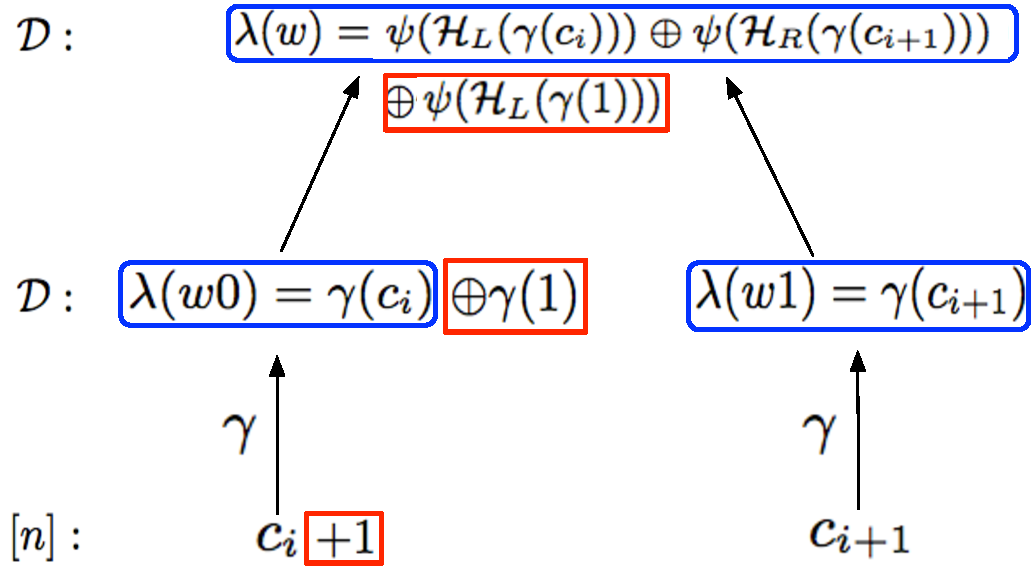
\includegraphics[scale = 0.4]{fig/update_illustrate.pdf}
\caption{Update of labels. At the leaf nodes $w0$ and $w1$, frequency values $c_{i}$ and $c_{i+1}$ are stored respectively. The labels of $w0$ and $w1$ are therefore $\gamma(c_{i})$ and $\gamma(c_{i+1})$. By Definition~\ref{main_expression}, the label of their parent node $w$ is $\psi ( {\cal H}_{L} ( \gamma (c_{i})))  \oplus \psi ( {\cal H}_{R} ( \gamma (c_{i+1}) ))$. Now, assume frequency value stored at leaf $w0$ is updated to $c_{i}+1$. The label of $w0$ can simply be updated by an $\oplus$ operation with $\gamma(1)$. Similarly, the label of $w$ is updated by an $\oplus$ operation with $\psi ( {\cal H}_{L} ( \gamma (1) ))$.}\label{label_update}
\end{figure}

\begin{defn}[Labeling function]\label{main_expression}
Let $T_\mathcal{C}$ be a structured binary tree, where $\mathcal{C}=[c_0, c_1, \ldots,c_{M-1}]$. For every node $w\in T_{\mathcal{C}}$, we define its labeling as $\lambda(w) ={\sum_{v\in \mathsf{range}(w)}} \mathcal{L}_w(v) \in {\mathcal{D}}$.
\end{defn}

E.g., Figure~\ref{label_update} illustrates a simple example of the labeling function. At the leaf level of a generalized hash tree, frequency values $c_{i}$ and $c_{i+1}$ are stored at leaf node $w0$ and $w1$. Hence, the labels of $w0$ and $w1$ are $\lambda(w0) = \gamma(c_{i})$ and $\lambda(w1) = \gamma(c_{i+1})$. By Definition~\ref{main_expression}, the label of their parent node $w$ should be the summation over ${\mathcal{D}}$ of the partial labels of $w$ with respect to $w0$ and $w1$. Hence, $\lambda(w) = \psi ( {\cal H}_{L} ( \gamma (c_{i})))  \oplus \psi ( {\cal H}_{R} ( \gamma (c_{i+1}) ))$.

%{\bf Constraint.} In a legitimate generalized hash tree, the labeling of each node must be in domain $\mathcal{D}$. Hence, our choices of hash function, projection function and $\gamma$ need to guarantee 
%\begin{equation}\label{constraint}
%\sum_{v\in \mathsf{range}(w)} \mathcal{L}_w(v) \in \mathcal{D} \text{,  for every node } w\in T_{\mathcal{C}}. 
%\end{equation}
%In~\cite{Papa}, function $\gamma$ is defined by $\gamma(c_{v}) = c_{v} \cdot {\bf 1}$. This setup, together with the projection function choice, ensures that every node labeling has a legitimate value in the domain.


%We now prove the following two important lemmas that we are going to use to prove the final result (generalized hash tree):

\begin{lemma}\label{property-2}
Let $T_\mathcal{C}$ be a structured binary tree. Let $h, \phi, \lambda$ be the hash function, projection function and labeling function described above. Then, $\phi(\lambda(w)) = h(\lambda(w{0}), \lambda(w{1}))$, where $w$ is any internal node of $T_\mathcal{C}$ and $w{0}, w{1}$ are two children of $w$.
\end{lemma}
\begin{proof}
\begingroup\makeatletter\def\f@size{7.5}\check@mathfonts
\def\maketag@@@#1{\hbox{\m@th\large\normalfont#1}}%
\begin{align*}
&\phi(\lambda(w))=\phi\left(\sum_{v\in \mathsf{range}(w)} \mathcal{L}_w(v)\in {\mathcal{D}} \right) 
\nonumber \text{\ \ (Def.~\ref{main_expression})}\\
&={\sum_{v\in \mathsf{range}(w0)} \phi\left(\mathcal{L}_w(v)\right)} \otimes \sum_{v\in \mathsf{range}(w1)}\phi\left(\mathcal{L}_w(v)\right) 
\nonumber \text{\ \ (Def.~\ref{hashfunction})}\\
&=\sum_{v\in \mathsf{range}(w0)}\phi\left(g_{w-v}(\gamma (c_v))\right) \otimes \sum_{v\in \mathsf{range}(w1)}\phi\left(g_{w-v}(\gamma(c_v))\right) 
\nonumber \text{\ \ (Def.~\ref{weight_of_a_node})}\\
%&=&\sum_{v\in \mathsf{range}(w0)}\phi\left(g_0(g_{w0-v}(\gamma(c_v)))\right)+\sum_{v\in \mathsf{range}(w1)}\phi\left(g_1(g_{w1-v}(\gamma(c_v)))\right)
%\nonumber \text{\ \ (Def.~\ref{compose_def})}\\
&=\sum_{v\in \mathsf{range}(w0)}\phi\left(g_0(\mathcal{L}_{w0}(v))\right) \otimes \sum_{v\in \mathsf{range}(w1)}\phi\left(g_1(\mathcal{L}_{w1}(v))\right) 
\nonumber \text{\ \ (Def.~\ref{weight_of_a_node})}\\
&=\sum_{v\in \mathsf{range}(w0)}\phi\left(\psi( {\bf {\cal H}_{L}} \cdot \mathcal{L}_{w0}(v))\right) \\
& \quad \quad \otimes \sum_{v\in \mathsf{range}(w1)}\phi \left(\psi({\bf {\cal H}_{R}} \cdot\mathcal{L}_{w1}(v))\right) 
\nonumber \text{\ \ (Def.~\ref{compose_def})}\\
&=\sum_{v\in \mathsf{range}(w0)} {\bf {\cal H}_{L}} \cdot\mathcal{L}_{w0}(v)
 \otimes \sum_{v\in \mathsf{range}(w1)}{\bf {\cal H}_{R}}\cdot\mathcal{L}_{w1}(v) 
\nonumber \text{\ \ (Cor.~\ref{phipsi})}\\
&={\bf {\cal H}_{L}} (\lambda(w0)) \otimes {\bf {\cal H}_{R}} (\lambda(w1)  ) =h(\lambda(w0), \lambda(w1)).
\nonumber \text{\ \ (Def.~\ref{main_expression})} 
\end{align*}\endgroup
\end{proof}
%\babis{you might want to put reference to definitions and relative corollaries back in}
\begin{theorem}\label{final_thm}
Let $T_\mathcal{C}$ be a structured binary tree. Then, $(T_\mathcal{C},\lambda,$\\
$f,h)$ is a generalized hash tree, where $h, \phi, \lambda$ are the hash function, projection function and labeling function described above. .
\end{theorem}
\begin{proof}
It follows from Lemma~\ref{property-2} and by Definition~\ref{def_generalized}. 
\end{proof}

\subsection{Efficient updates of the labels}
The output $\lambda(v)$ of the labeling function applied to node $v$ can be updated very efficiently whenever the leaf changes. We first introduce the following definition.
\begin{defn}[Unit update]\label{delta}
For any internal node $w \in T_{\mathcal{C}}$ and any leaf node $v \in T_{\mathcal{C}}$, let the unit update of $w$ in terms of $v$ be $\delta_w(v) = g_{\epsilon - v_{i}}(\gamma(1))$.
\end{defn}
Each occurrence of an element $i$ contributes $\delta_w(i)=g_{w - v_{i}}(\gamma(1))$ on the internal node $w$. Adding (or removing) an element $i$ is equivalent to adding (or subtracting) $\delta_w(i)$ to (from) $\lambda(w)$. It is important to note that computing a unit update, as well as a partial label, only requires $O(\log M)$ recursive calls of hash function $h$. 

Figure~\ref{label_update} shows how to update the corresponding labels when the value stored at leaf node $w0$ increments by $1$. For a more concrete example, let $\lambda(\epsilon)$ be the label of the root of a generalized hash tree $(T_{\mathcal{C}},\lambda,\phi,h)$ with eight leaves $\{v_{0},v_{1},\ldots,v_{7}\}$ where $c_3=2$, $c_4=c_6=c_7=1$ and $c_0=c_1=c_2=c_5=0$. By Corollary~\ref{prune}, the root label $\lambda(\epsilon) = \sum_{v\in \mathsf{range}(\epsilon)} \mathcal{L}_w(v)\in {\mathcal{D}}$ can be expressed as $ \mathcal{L}_\epsilon(v_{2})+\mathcal{L}_\epsilon(v_{4})+\mathcal{L}_\epsilon(v_{6})+\mathcal{L}_\epsilon(v_{7})$. Adding (or removing) an element $i$ is equivalent to adding (or subtracting) $\delta_\epsilon(i)$ to (from) $\lambda(\epsilon)$, which only takes $O(\log M)$ calls of $h$.
\subsection{SADS construction}\label{streaming_dictionary}
Let $T_{\mathcal{C}}$ be a structured binary tree with $M$ leaves corresponding to the universe. Let $(T_{\mathcal{C}},\lambda,\phi,h)$ denote the generalized hash tree of interest as described above. To store the generalized hash tree, we store only the labels that are defined on the paths from non-zero leaves to the root (all other labels are zero). This requires space proportional to $O(\nu \log M)$, where $\nu$ is the number of distinct element appearing in the stream. Figure~\ref{algorithms_sads} presents the 6 algorithms of our abstract SADS scheme. 


{\bf Range search queries.}
The abstract SADS inherits the query expressiveness from the PSTY work~\cite{DBLP:conf/eurocrypt/PapamanthouSTY13}. It supports the range search queries by the same algorithm.

 The proof for a range search query $[x,y]$ simply contains the two proofs $\Pi(x)$ and $\Pi(y)$ as output by algorithms $\mathsf{query}(x,D_h,\mathsf{auth}$\\
 $(D_h),\mathsf{pk})$ and $\mathsf{query}(y,D_h,\mathsf{auth}(D_h),\mathsf{pk})$ respectively from Figure~\ref{algorithms_sads}. It also contains the frequencies $\mathcal{C}_{xy}=\{c_{a_1},c_{a_2},\ldots,c_{a_s}\}$ of the reported range as an answer. Let now $\mathcal{R}_{xy}=\{a_1,a_2,\ldots,a_s\}$ denote the respective reported range that corresponds to $\mathcal{C}_{xy}$.

%\frame box[2.8][l]{{\bf Algorithm} $\mathsf{pk}\leftarrow\mathsf{genkey}(1^\lambda,n)$: } \par

\begin{figure*}[ht!]
{
\centering
\framebox{\parbox{0.99\textwidth}{
\paragraph{\textbf{Algorithm}  $\mathsf{pk}\leftarrow\mathsf{genkey}(1^\lambda,n)$} On input the security parameter $\lambda$ and a bound $n$ on the size of the stream, set $\mathsf{pk}=\{\vc{L},\vc{R},{\cal U}\}$, where ${\cal U}$ is a universe such that $|{\cal U}|=M$ and $\vc{L},\vc{R}$ specify the hash function.
}}} 
%\newline\newline
{\centering
\framebox{\parbox{0.99\textwidth}{
\paragraph{\textbf{Algorithm}  $\{\mathsf{auth}(D_0),d_0\}\leftarrow\mathsf{initialize}(D_0,\mathsf{pk})$} Let $D_0$ be a structured binary tree $T_\mathcal{C}$ where $c_i=0$ ($i=0,\ldots,M-1$). The algorithm outputs the generalized hash tree $(T_{\mathcal{C}},\lambda,\phi,h)$ as $\mathsf{auth}(D_0)$, where $\lambda(v)={\bf 0_{\mathcal{D}}}$ for all nodes $v$ in $T_{\mathcal{C}}$. Also it outputs $d_0={\bf 0_{\mathcal{D}}}$. 
}}}
{\centering
\framebox{\parbox{0.99\textwidth}{
\paragraph{\textbf{Algorithm}  $d_{h+1}\leftarrow\mathsf{updateVerifier}(x,d_h,\mathsf{pk})$} Let $x\in {\cal U}$ be the current element of the stream. The algorithm updates the local state by setting $d_{h+1}=d_h \oplus \delta_{\epsilon}(x)$, where $\epsilon$ is the root of $T_{\mathcal{C}}$ and $\delta_{\epsilon}(x)$ is defined in Definition~\ref{delta}.%and $\vc{1}$ is the unit vector of $k$ entries.
}}}
{\centering
\framebox{\parbox{0.99\textwidth}{
\paragraph{\textbf{Algorithm} $\{D_{h+1},\mathsf{auth}(D_{h+1})\}\leftarrow\mathsf{updateProver}(x,D_h,\mathsf{auth}(D_h),\mathsf{pk})$}
Let $x\in {\cal U}$ be the current element of the stream. The algorithm sets $c_x=c_x+1$, outputting the updated tree $T_{\mathcal{C}}$. Let $v_{\ell},\ldots,v_1$ be the path in $T_{\mathcal{C}}$ from node $v_{\ell}$ ($v_{\ell}$ stores $c_x$) to the child $v_1$ of the root $\epsilon$ of $T_{\mathcal{C}}$. Set
\begin{equation}\label{structure_update}
\lambda(v_i)=\lambda(v_i) \oplus \delta_{v_{i}}(x) \text{\ for $i=\ell,\ell-1,\ldots,1$}\,,
\end{equation}
where $\delta_{v_{i}}(x)$ is defined in Definition~\ref{delta}. The new authenticated data structure $\mathsf{auth}(D_{h+1})$ is the new generalized hash tree with the updated labels as computed in Equation~\ref{structure_update}.
}}}
{\centering
\framebox{\parbox{0.99\textwidth}{
\paragraph{\textbf{Algorithm} $\{\alpha(q),\Pi(q)\}\leftarrow\mathsf{query}(q,D_h,\mathsf{auth}(D_h),\mathsf{pk})$} Let $q$ be a frequency query for element $x\in {\cal U}$. Set $\alpha(q)=c_x$ (note that if $c_x=0$, $x$ is not contained in the collection). Let $v_{\ell},\ldots,v_1$ be the path in the structured binary tree $T_{\mathcal{C}}$ from node $v_{\ell}$ ($v_{\ell}$ stores the value $c_x$) to the child $v_1$ of the root $\epsilon$ of $T_{\mathcal{C}}$. Let also $w_{\ell},\ldots,w_1$ be the \emph{sibling nodes} of $v_{\ell},\ldots,v_1$. Proof $\Pi(q)$ contains the ordered sequence of the pairs of labels belonging to the tree path from leaf $v_\ell$ to the root $\epsilon$ of the tree, i.e., the pairs $\{(\lambda(v_{\ell}),\lambda(w_{\ell})),(\lambda(v_{\ell-1}),\lambda(w_{\ell-1})),\ldots,(\lambda(v_{1}),\lambda(w_{1}))\}$.
}}}
{\centering
\framebox{\parbox{0.99\textwidth}{
\paragraph{\textbf{Algorithm} $\{{\tt{1}},{\tt{0}}\}\leftarrow
  \mathsf{verify}(q,\alpha(q),\Pi(q),d_h,\mathsf{pk})$} Let $q$ be a frequency query for element $x\in {\cal U}$. Parse $\Pi(q)$ as $$\{(\lambda(v_{\ell}),\lambda(w_{\ell})),\ldots,(\lambda(v_{1}),\lambda(w_{1}))\}$$ and $\alpha(q)$ as $c_x$. 

If $\lambda(v_{\ell})\ne \gamma(c_x) $ or $\lambda(v_{\ell}),\lambda(w_{\ell}) \notin {\mathcal{D}}$, output ${\tt{0}}$. Compute values $y_{\ell-1},y_{\ell-2},\ldots,y_0$ as $y_i=h(\lambda(v_{i+1}), \lambda(w_{i+1}))$ (if $v_{i+1}$ is $v_{i}$'s left child) or $y_i=h(\lambda(v_{i+1}),\lambda(w_{i+1}))$ (if $v_{i+1}$ is $v_{i}$'s right child). For $i=\ell-1,\ldots,1$, if $\phi(\lambda(v_i))\ne y_i$ \textbf{or} $\lambda(v_i),\lambda(w_i)\notin {\mathcal{D}}$ output ${\tt{0}}$. If $\phi(d_h)\ne y_0$, output ${\tt{0}}$. Output ${\tt{1}}$.
}}}
%\newline
\footnotetext{If $v_{i+1}$ is $v_{i}$'s right child, we set $y_{i}=\vc{R}\cdot\lambda(v_{i+1})+\vc{L}\cdot\lambda(w_{i+1})$.}
\caption{\label{algorithms_sads}Algorithms of the abstract SADS for verifying frequency queries.}
\end{figure*}


For verification, the proofs $\Pi(x)$ and $\Pi(y)$ are verified first by using algorithm $\mathsf{verify}$ from Figure~\ref{algorithms_sads}. If this verification is successful, perform the following test (else reject): If for all labels $\lambda(v)\in \Pi(x) \cup \Pi(y)$ such that $\mathsf{range}(v)\cap\mathcal{R}_{xy}$ is not empty, the following relation (as in Definition~\ref{main_expression}) 
\begin{equation}\label{eq:check_efficiency}
\lambda(v) =\sum_{i\in \mathsf{range}(v)\cap\mathcal{R}_{xy}} \mathcal{L}_v(i)
\end{equation}
is true, output $\tt{1}$ (i.e., accept), else output $\tt{0}$ (i.e., reject).
The above relation ensures that all the range (with the correct frequencies) has been reported, or otherwise, the adversary could find a collision. The above technique can be also used for verifying successor queries, where the reported range is empty.

\subsection{PSTY instantiation of our abstract SADS}\label{instantiation}
We show the PSTY scheme~\cite{DBLP:conf/eurocrypt/PapamanthouSTY13} is an instantiation of our abstract SADS. Recall our SADS is built upon a generalized hash tree $(T,\lambda,\phi,h_{old})$, where $h_{old}$ is a collision resistant hash function, $\phi$ is a projection function and $\lambda$ is a labeling function. In particular, the labeling function $\lambda$ is determined by the hash function $h_{old}$, the $\gamma$ function and the inverse projection function $\psi$. We next study all four components of the PSTY scheme~\cite{DBLP:conf/eurocrypt/PapamanthouSTY13}.

{\bf Hash function.} 
The hash function $h_{old}$ uses ${\mathcal{D}}= \mathbb{Z}_n^{t}$ and ${\mathcal{R}} = \mathbb{Z}_q^{\nu}$ as its domain and range. The operation $\oplus$ of ${\mathcal{D}}$ is mod $n$ addition, and the operation $\otimes$ of ${\mathcal{R}}$ is mod $q$ addition. 
Specificially, $h_{old}$ is defined as: 
\begin{enumerate}
\item $h_{old} ({\bf x, y})= {\bf {\cal H}_{L}(x)}  + {\bf {\cal H}_{R}(y)}$ mod q;
\item ${\bf {\cal H}_{A}(x)} = {\bf A \cdot x}$ mod q, where $\bf A= L, R$ is a randomly picked matrix from $\mathbb{Z}_q^{\nu \times t}$.
\end{enumerate}
${\bf {\cal H}_{A}}$ is collision resistant based on the hardness assumption of the small integer solution problem $\mathsf{SIS}_{q, t,\beta}$~\cite{DBLP:journals/siamcomp/MicciancioR07}. Here, $q$ is a large prime, $t=\nu \lceil \log q \rceil$, $\beta$ is set to $n\sqrt{2t}$.

First, we show $h_{old}$ is collision resistant. Assume there exist $\bf x_{\delta}, y_{\delta} \neq 0_{\mathcal{D}}$ such that $\bf {\cal H}_{L}(x_{\delta}) + {\cal H}_{R}(y_{\delta})= {\bf 0}_{\mathcal{R}}$ with non-negligible probability. This would give a solution to $\mathsf{SIS}_{q, 2t,\beta}$ with the matrix be $[L,\, R]$ randomly chosen from $\mathbb{Z}_q^{\nu \times 2t}$. 


%Let $q$ be a large enough prime, $t=\lambda \lceil \log q \rceil$ and $\beta=n\sqrt{2t}$. The hash function $h_{old}$ uses ${\mathcal{D}}= \mathbb{Z}_n^{t}$ and ${\mathcal{R}} = \mathbb{Z}_q^{\lambda}$. The operation $\oplus$ of ${\mathcal{D}}$ is mod $n$ addition, and the operation $\otimes$ of ${\mathcal{R}}$ is mod $q$ addition. 
%Specificially, $h_{old}$ is defined as: 
%\begin{enumerate}
%\item $h_{old} ({\bf x, y})= {\bf {\cal H}_{L}(x)}  + {\bf {\cal H}_{R}(y)}$ mod q;
%\item ${\bf {\cal H}_{A}(x)} = {\bf A \cdot x}$ mod q, where $\bf A= L, R$ is a randomly picked matrix from $\mathbb{Z}_q^{\lambda \times t}$.
%\end{enumerate}
%First, ${\bf {\cal H}_{A}}$ is collision resistant based on the hardness assumption of the small integer solution problem $\mathsf{SIS}_{q, t,\beta}$~\cite{DBLP:journals/siamcomp/MicciancioR07}. Assume there exist $\bf x_{\delta}, y_{\delta} \neq 0_{\mathcal{D}}$ such that $\bf {\cal H}_{L}(x_{\delta}) + {\cal H}_{R}(y_{\delta})= {\bf 0}_{\mathcal{R}}$ with non-negligible probability. But this would give a solution to $\mathsf{SIS}_{q, 2t,\beta}$ with the matrix be $[L,\, R]$ in $\mathbb{Z}_q^{\lambda \times 2t}$. Hence, $h_{old}$ is collision resistant.

Second, given ${\bf x, y} \in {\mathcal{D}}$ such that ${\bf x + y} \in {\mathcal{D}}$, it is obvious that $${\bf {\cal H}_{A}(x \oplus y)} = {\bf {\cal H}_{A}(x + y)} = {\bf A \cdot x} + {\bf A \cdot y} \text{  mod q}.$$The labeling function below ensures that for any two labels ${\bf x, y} \in {\mathcal{D}}$ in the generalized hash tree, ${\bf x + y} \in {\mathcal{D}}$ holds. 

From the above two arguments, $h_{old}$ meets the characterization of Definition~\ref{hashfunction}.

{\bf Projection function.}
The projection function $\phi: \mathbb{Z}_n^{t} \rightarrow \mathbb{Z}_q^\nu$ \emph{parses} the input vector $\vc{x}$ as a radix-2 representation (i.e., a base-2 representation but not necessarily of binary coefficients) and converts it to the respective vector in $\mathbb{Z}_q^\nu$. 

On input a vector $\vc{x}\in \mathbb{Z}_n^{t}$, where $\tau = \lceil \log q \rceil$ and $t=\nu \cdot \tau$, output a vector $\vc{y} = \phi(\vc{x})$ of $\nu$ entries such that each $\vc{y}_i$ ($i=0,\ldots,\nu-1$) is the number in $\mathbb{Z}_q$ represented by the radix-2 representation $[\vc{x}_{i\tau},\vc{x}_{i\tau+1},\ldots,\vc{x}_{(i+1)\tau-1}]^{\mathsf{T}}$, namely $$\vc{y}_i=\sum_{j=0}^{\tau-1}\vc{x}_{i\tau +j}2^j\mod q\,,\text{ for $i=0,\ldots,\nu-1$}\,.$$

It is easy to check that $\phi$ here forms a surjective homomorphism from $\mathbb{Z}_n^{t}$ to $\mathbb{Z}_q^\nu$. 

{\bf Inverse projection function.}
The inverse projection function $\psi: \mathbb{Z}_q^\nu \rightarrow \mathbb{Z}_n^{t}$ is simply the binary representation of vectors. For example, if $\nu=2$, $q=8$ and $\vc{a}=[6,3]^{\mathsf{T}}\in \mathbb{Z}_8^2$, then $\psi (\vc{a})=[1,1,0,0,1,1]^{\mathsf{T}}$, since $\psi(6)=[1,1,0]^{\mathsf{T}}$ and  $\psi(3)=[0,1,1]^{\mathsf{T}}$. Obviously, $\psi$ here satisfies Definition~\ref{inverseprojection}.

{\bf $\gamma$ function. }
The gamma function $\gamma: [n] \rightarrow \mathbb{Z}_n^{t}$ is defined as:
\begin{equation}\label{gamma1}
\gamma(c_{v}) = c_{v} \cdot {\bf 1}, 
\end{equation}
where $\vc{\emph{1}}= [1, 1, \ldots, 1]^{\mathsf{T}} \in \mathbb{Z}_n^{t}$. Clearly, $\gamma(c_{v1}+c_{v2}) = \gamma(c_{v1}) + \gamma(c_{v2})$ mod n, given $c_{v1}+c_{v2} \in [n]$. 

Let $T_{C}= (T, \lambda, \phi, h_{old})$ be the generalized hash tree as described above. For any node $w \in T_{C}$, by Definition~\ref{main_expression} we have its label $\lambda(w) ={\sum_{v\in \mathsf{range}(w)}} \mathcal{L}_w(v) \in {\mathcal{D}}$ . Since the entries of each partial label $\mathcal{L}_w(v) = c_{v} \cdot \{0,1\}^{t}$ and $\sum_{i=0}^{M-1}c_i\le n$, we know $\lambda(w)\in \mathbb{Z}_{n}^t$. It follows that for any two labels ${\bf x, y} \in T_{C}$, ${\bf x+y}  \in \mathbb{Z}_{n}^t$ is also true. Therefore, $T_{C}$, as it is described in PSTY~\cite{DBLP:conf/eurocrypt/PapamanthouSTY13}, is an instance of the abstract SADS.

In the following sections, we show how to build an improved instantiation of the abstract SADS by employing a better hash function. The choices of the {\it projection function}, the {\it inverse projection function} and {\it $\gamma$ function} {\bf remain the same}.
%We now give our final result stating the formal security guarantee of our algorithms, along with their detailed asymptotic performance. The correctness of our scheme follows easily by inspecting the algorithms, therefore its proof is omitted. The security proof and the proof of asymptotic performance are in the Appendix.
%\begin{theorem}[Streaming authenticated frequency with range search]\label{main_theorem_lattice}
%Let $k$ be the security parameter, $n=\mathsf{poly}(k)$ be an upper bound on the size of a stream containing elements from an ordered universe $\mathcal{U}$ of size $M$, $\{q,\mu,\beta\}\leftarrow {\sf parameters}(1^k,n)$ and $\nu$ be the number of unique elements that have appeared in the stream. There exists a streaming authenticated data structure scheme for one-dimensional frequency queries and one-dimensional range queries (outputting the respective frequencies) such that: \textbf{(a)} It is correct according to Definition~\ref{sound_def} and secure according to Definition~\ref{sec_def_general} and assuming hardness of $\mathsf{SIS}_{q,\mu,\beta}$ (Assumption~\ref{assume_sis}); \textbf{(b)} Algorithms $\mathsf{updateVerifier}$ and $\mathsf{updateProver}$ run in $O(\log M\log^2 n)$ time; \textbf{(c)} Algorithm $\mathsf{query}$ (both for frequency and range search queries) runs in $O(\log M\log n)$ time, outputting a proof of size $O(\log M\log n)$; \textbf{(d)} A frequency query can be verified in $O(\log M\log ^2 n)$ time and a range search query can be verified in $O(s\log M\log ^2 n)$ time, where $s$ is the size of the output range; \textbf{(e)} The space required at the verifier is $O(\log n)$ and the space required at the prover is $O(\nu\log M\log n)$. 
%\end{theorem}

%Our algorithms can be extended to two (or multiple) dimensions by leveraging existing methods for multidimensional range queries~\cite{DBLP:journals/algorithmica/MartelNDGKS04}, carefully adjusted in our framework. Due to space limitations, we defer such extensions to the full version of our paper.










